\section{Decodificação da Instrução}
	\subsection{Diagrama de Classe}
  \begin{figure}[H]
    \begin{center}
	\begin{tikzpicture}
	\umlclass[x=0,y=0]{Instruction Decode}{
	+ clock : input bit \\
	+ reset : input bit \\
	+ instruction : input bit[32] \\ 
	+ regDst : input bit[5] \\
	+ writeData : input bit \\
	+ writeRegister : input bit[5] \\
	+ word : input bit[16] \\
	+ branch : output bit \\
	+ memRead : output bit \\
	+ memToReg : output bit \\
	+ aluOp : output bit[2] \\
	+ memWrite : output bit \\
	+ aluSrc : output bit \\
	+ regWrite : output bit \\
	+ jump : output bit \\
	%+ readData1 : output bit[32] \\
	%+ readData2 : output bit [32] \\
	%+ outputWord : output bit [32] \\
	- registers : reg bit[32] \\}			
	{ % procedures
          - \underline{<<comb>> opcode\_decoder()} \\
          - <<comb>> search\_register() \\
          - <<comb>> set\_write\_register() \\
          - <<sequ>> sign\_extend() \\
          - <<sequ>> zero\_extend()
        }
	\end{tikzpicture}
\end{center}
  \end{figure}
		
		\subsection{Definições de entrada e saída}
		
	\begin{center}
		\begin{longtable}[pos]{| l | c | c | m{7cm} |} \hline
			\multicolumn{1}{|c|}{\cellcolor[gray]{0.9}\textbf{Nome}} & 
			\multicolumn{1}{c|}{\cellcolor[gray]{0.9}\textbf{Tamanho}} & 
			\multicolumn{1}{c|}{\cellcolor[gray]{0.9}\textbf{Direção}} &
			\multicolumn{1}{c|}{\cellcolor[gray]{0.9}\textbf{Descrição}} \\ \hline
			\endhead
			\hline
			\endlastfoot
			
			instruction & 1 & entrada & Instrução a ser executada. \\ \hline
			writeData & 32 & entrada & Sinal de controle para escrita no registrador. \\ \hline
			writeRegister & 32 & entrada & Endereço do registrador de destino do writeData. \\ \hline
			word & 32 & entrada & é uma instrução. \\ \hline
			branch & 32 & saída & Sinal que informa ao circuito se a instrução é de branch. \\ \hline
			memRead & 32 & saída & Sinal de controle para realizar leitura da memória. \\ \hline
			memToReg & 32 & saída & Sinal de controle que define se o dado deve vir da ULA ou da memória \\ \hline
			aluOp & 32 & saída & Sinal de controle que define se o código funct da instrução deve ser levado em consideração ou não. \\ \hline
			memWrite & 32 & saída & Sinal de controle para realizar escrita na memória. \\ \hline
			aluSrc & 32 & saída & Sinal de controle que define qual entrada a ULA deve utilizar para realizar a operação. \\ \hline
			regWrite & 32 & saída & Sinal de controle para realizar escrita no registrador. \\ \hline
			jump & 32 & saída & Sinal que informa ao circuito se a operação é de jump. \\ \hline
		\end{longtable}
	\end{center}
	
	\subsection{Datapath Interno}
	
%	\begin{figure}[ht]
%		\begin{center}
%		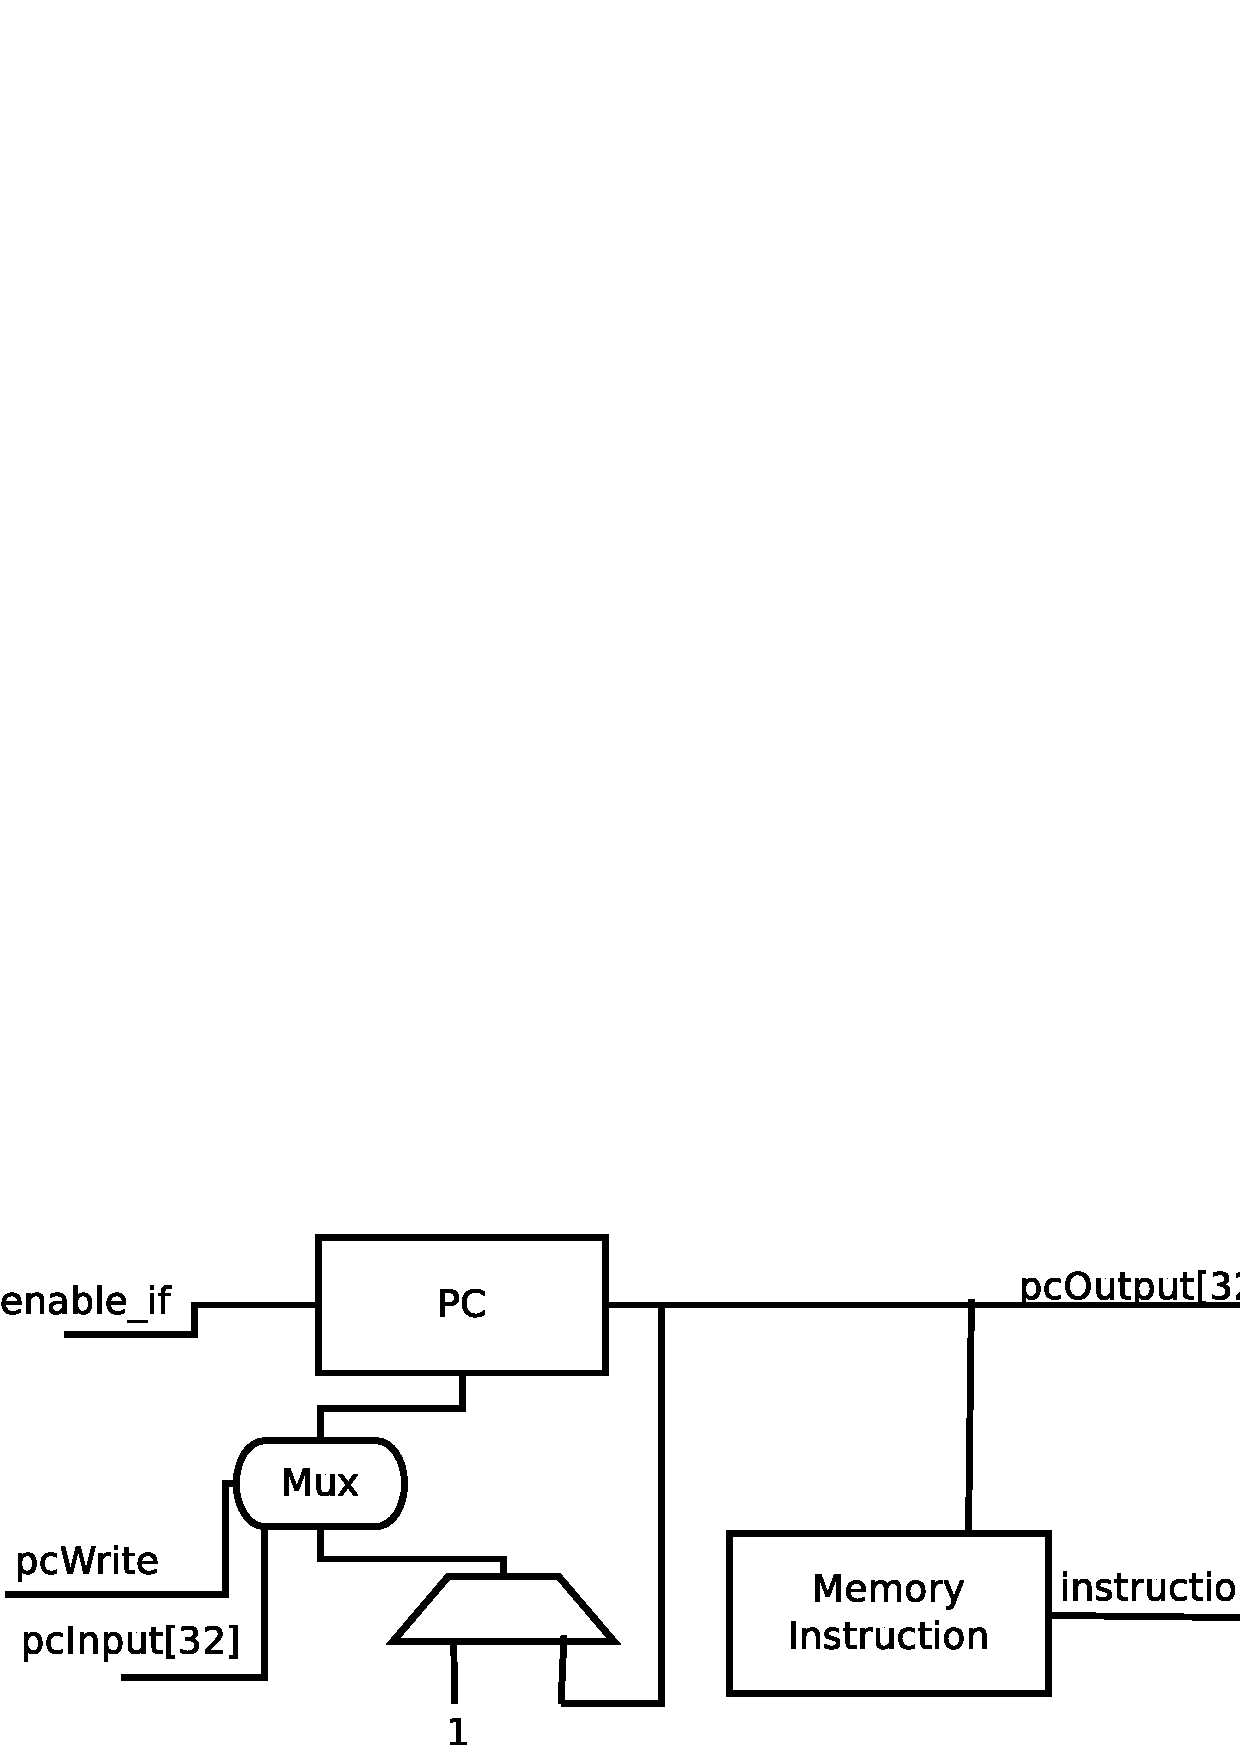
\includegraphics{./datapath/step1.jpg}
%		\caption*{Datapath preliminar}
%		\end{center}
%	\end{figure}